% !TeX program = xelatex
\providecommand{\PaperRoot}{./}
\makeatletter\edef\input@path{{\PaperRoot}{\PaperRoot template/}}\makeatother
\documentclass[a4paper,12pt,review]{cas-sc}
\geometry{a4paper,margin=25mm}
\makeatletter\@fleqnfalse\makeatother
\usepackage[numbers,sort&compress]{natbib}
\usepackage{bm,tabularx,longtable,placeins,float}
\hypersetup{hidelinks}
\graphicspath{{\PaperRoot}}
\newcommand{\R}{\mathbb R}\newcommand{\C}{\mathbb C}
\newcommand{\Rea}{\operatorname{Re}}\newcommand{\tr}{\operatorname{tr}}
\setlength{\emergencystretch}{2em}
\ExplSyntaxOn
\RenewDocumentCommand\MaketitleBox{O{}}
 {\group_begin:\use:c{@title}\par\group_end:\vspace{12pt}}
\cs_set_protected:Npn\__make_tbl_caption:nn #1#2
 {\l_tbl_align_tl\skip_vertical:N\l_tbl_abovecap_skip
  \parbox{\l_tbl_width_dim}{\centering\sffamily\small\textbf{#1}\par #2\par\vskip4pt}
  \skip_vertical:N\l_tbl_belowcap_skip}
\cs_set_protected:Npn\__make_fig_caption:nn #1#2
 {\l_fig_align_tl\skip_vertical:N\l_fig_abovecap_skip
  \parbox{\l_fig_width_dim}{\centering\sffamily\small\textbf{#1:}~#2\par}
  \skip_vertical:N\l_fig_belowcap_skip}
\cs_set:Npn\__first_footerline:{\small\rmfamily\itshape Supplementary~material}
\cs_new_eq:NN\paper_printorcid:\printorcid
\RenewDocumentCommand\printorcid{} {\seq_if_empty:NF\g_stm_orcid_seq{\paper_printorcid:}}
\ExplSyntaxOff
\begin{document}
\let\WriteBookmarks\relax
\shorttitle{Supplement: direct localization of overlapping wideband sources}
\shortauthors{}
\title[mode=title]{Supplementary material: Efficient direct localization of overlapping wideband sources with unequal powers}
\maketitle
\renewcommand{\thesection}{S\arabic{section}}
\numberwithin{equation}{section}\numberwithin{figure}{section}\numberwithin{table}{section}

\section{Reproduction data and new source coordinates}
The main paper compares a common 240-observation subset, an expanded 2,400-observation cohort containing that subset, and 480 observations from 16 new source configurations. The curvature comparison reuses the common 240 observations. These counts describe different comparison duties and are not added as independent data. All use the same four receiver coordinates; a new configuration changes source positions, not the receiver array.

Table~\ref{sup:coordinates} supplies the new source coordinates in meters, rounded to six decimal places. The accompanying \texttt{data/submission/new\_layouts.csv} retains the saved numerical precision. Configuration numbers are one-based here: the zero-based stored layout is the displayed number minus one. Categories 1--4 mean both inside, A outside/B inside, A inside/B outside, and both outside the receiver convex hull. The geometry and waveform generation seeds are 20261020071 and 20261020072. Realization identifiers are 1000--1004. The geometry constraints are minimum distances of 150 m to a receiver, 100 m to the origin and 50 m to any station-pair line, with at least 300 m between sources. No configuration is screened by localization outcome.
\begin{table}[pos=H]\centering\small
\caption{New source coordinates (m). A is the power-scaled source and B the fixed-power source.}\label{sup:coordinates}
\begin{tabular}{@{}rrrrrr@{}}\toprule
No. & Category & $x_A$ & $y_A$ & $x_B$ & $y_B$\\\midrule
1 & 1 & -209.742960 & -211.672998 & -135.426339 & 121.578497\\
2 & 1 & -115.361316 & 76.809910 & 67.769590 & -192.728293\\
3 & 1 & -208.559801 & 115.499630 & 268.616751 & -92.726639\\
4 & 1 & 173.459164 & -110.441904 & -168.154517 & -145.923194\\
5 & 2 & -926.529606 & 771.380729 & -198.481435 & 152.456653\\
6 & 2 & -628.314566 & -929.843027 & -55.519139 & -297.939120\\
7 & 2 & -195.757938 & -496.419920 & 157.528284 & 224.885259\\
8 & 2 & -734.894082 & -306.033731 & -249.535479 & 71.485648\\
9 & 3 & -64.564529 & 351.783227 & 663.100329 & 428.023655\\
10 & 3 & -166.451414 & 260.105867 & 823.995321 & 431.176047\\
11 & 3 & 74.808116 & 299.580428 & -702.622192 & 474.464614\\
12 & 3 & -162.472651 & -112.907043 & 765.537745 & -808.531366\\
13 & 4 & 313.792247 & 602.900501 & 700.222844 & -274.728424\\
14 & 4 & 482.010461 & 239.752856 & 888.180085 & 90.857032\\
15 & 4 & -374.838719 & 599.269525 & 240.800462 & 663.866438\\
16 & 4 & 624.598019 & 542.011213 & -163.287363 & 904.989973\\\bottomrule
\end{tabular}\end{table}
\FloatBarrier

\section{Baseline objectives and finite-window consistency}
\subsection{Single-source LS, wideband MUSIC and MVDR-known}
All responses use the main paper's known relative-amplitude and baseband-delay model. Unit-norm response $\bm q_f(\bm p)=\bm a_f(\bm p)/\|\bm a_f(\bm p)\|$ preserves relative station amplitudes. The LS baseline takes peaks from the single-source score and refines them continuously; it does not optimize a full two-source fit.

For covariance-based methods, split the same record into $S$ nonoverlapping segments, each with $N_s=N/S$ samples. Let $\bm z_{bf}\in\C^L$ be the segment DFT at physical frequency $f$, normalized by $1/N_s$, and let $F_s$ denote the retained frequency count on that segment grid. Then
\begin{equation}
\widehat{\bm C}_f=S^{-1}\sum_{b=1}^S\bm z_{bf}\bm z_{bf}^H.
\end{equation}
The assumed zero mean makes correlation and covariance equal. Segment noise variance is $\sigma_t^2/N_s$, whereas full-record noise variance is $\sigma_t^2/N$. Snapshots are never pooled across different realizations. Segmentation trades frequency resolution and segment duration for more same-frequency statistical samples.

MUSIC requires $K<L$, linearly independent source responses, full-rank source coefficient covariance and spatially white noise \cite{WeissAmar2005}. Independent sources with nonzero power satisfy the population source-rank requirement, but finite-sample subspace accuracy still depends on power imbalance and effective snapshots. Let $\bm E_{n,f}$ contain the $L-K$ eigenvectors associated with the smallest covariance eigenvalues. The implemented wideband score is
\begin{align}
S_{\rm MU}(\bm p)&=\left[\sum_f w_f\bm q_f^H\bm E_{n,f}\bm E_{n,f}^H\bm q_f\right]^{-1},\\
\widetilde w_f&=\max\{\tr(\widehat{\bm C}_f)-L\sigma_t^2/N_s,0\},
\qquad w_f=\widetilde w_f/\sum_v\widetilde w_v.
\end{align}
Uniform weights are used if all $\widetilde w_f$ vanish. Only retained-band bins are decomposed. Known $K$ determines subspace dimension; it does not guarantee that both signals are resolvable at every bin in a finite record.

MVDR minimizes output power subject to unit response \cite{Capon1969}. With loading
\begin{equation}
\bm C_{f,\delta}=\widehat{\bm C}_f+
 \delta\,\tr(\widehat{\bm C}_f)\bm I/L,
\end{equation}
the constraint $\bm h_f^H\bm q_f=1$ gives output power
$[\bm q_f^H\bm C_{f,\delta}^{-1}\bm q_f]^{-1}$, where $\bm h_f\in\C^L$ is the complex combining vector. The registered score is
\begin{equation}
S_{\rm MV}(\bm p)=F_s^{-1}\sum_f
 [\bm q_f(\bm p)^H\bm C_{f,\delta}^{-1}\bm q_f(\bm p)]^{-1}.
\end{equation}
The dimensionless $\delta$ multiplies mean diagonal covariance power. The suffix ``known'' identifies use of known relative propagation responses. This wideband score is not presented as the original DPD-HR formula \cite{TirerWeiss2016}.

\subsection{Full AP, multistart ML and GA-ML}
Full AP repeats global conditional searches and continuous position refinement, accepting by the joint waveform-eliminated residual \cite{ChenHudsonYao2002}. It uses up to six outer cycles and five candidates, retaining saved early outputs as well as final outputs. The final cost includes its additional checks.

Multistart ML optimizes the same four-dimensional joint objective from eight unique starts: four single-source spectral peak combinations and four Sobol spatial coverage starts. Unordered duplicate pairs are removed before optimization. GA-ML encodes the four coordinates as one real-valued individual. It uses tournament selection of size three, simulated binary crossover probability 0.9 and distribution index 15, polynomial mutation probability 0.25 per coordinate and index 20, and four elites \cite{DebAgrawal1995}. Population size is 128; the generation cap is 200, with stopping after 30 stagnant generations. Final joint continuous refinement is included in its cost. These are search implementations of the joint objective rather than different likelihood principles.

\subsection{Multi-frequency shared-power SBL}
For dictionary positions $\bm g_j$, define $\bm D_f=[\bm q_f(\bm g_1),\ldots,\bm q_f(\bm g_G)]$. SBL assumes frequency coefficients $\bm z_f\sim\mathcal{CN}(0,\bm\Gamma)$ with $\bm\Gamma=\operatorname{diag}(\bm\gamma)$, $\bm\gamma\ge0$, shared across frequencies \cite{Nannuru2019}. The covariance, posterior mean and negative log evidence are
\begin{align}
\bm C_f&=\sigma_f^2\bm I+\bm D_f\bm\Gamma\bm D_f^H,\\
\bm\mu_f&=\bm\Gamma\bm D_f^H\bm C_f^{-1}\bm x_f,\\
\mathcal E(\bm\gamma)&=F^{-1}\sum_f
 [\log\det\bm C_f+\bm x_f^H\bm C_f^{-1}\bm x_f].
\end{align}
The implementation uses the fixed-point update
\begin{equation}
\gamma_j^+=\gamma_j\left[
\frac{\sum_f|\bm d_{fj}^H\bm C_f^{-1}\bm x_f|^2}
{\sum_f\bm d_{fj}^H\bm C_f^{-1}\bm d_{fj}}
\right]^{1/2},
\end{equation}
with evidence backtracking. Every five iterations, eight active points undergo off-grid optimization: displacement is limited to 20 m per coordinate, coordinates are scaled by 1,000 m, and L-BFGS-B uses at most 20 iterations. Output peaks use individual $\gamma_j$ values. The run cap is 300 iterations. Every five iterations, stopping requires normalized evidence change below $10^{-5}$, relative $\ell_1$ change of $\gamma$ below 1\%, and maximum motion of outputs and active atoms below 0.05 m, on two consecutive checks. This displacement is an optimization stability threshold, not a localization accuracy requirement. The paper does not use the earlier aggregation-output branch.

\subsection{Finite-window diagnostic}
Four development configurations at 0 and 15 dB supply eight observations with stored clean source components. At true positions, define the model residual and expected projected noise energy
\begin{equation}
E_{\rm win}=\sum_{b,f}\|\bm\Pi_{\bm A_f}^{\perp}\bm z_{bf}^{(0)}\|^2,
\qquad E_n=SF_s(L-K)\sigma_t^2/N_s.
\end{equation}
All $\bm A_f$ are checked to have full column rank. The clean-data residual fractions for one, four and eight segments are respectively 0.209--0.382\%, 0.756--1.387\% and 1.529--2.854\%; their $E_{\rm win}/E_n$ ranges are 0.035--0.882, 0.126--3.210 and 0.238--6.611. Shorter segments increase common-window mismatch.

Rectangular, periodic Hann and 4,096-sample Hann windows with four overlapping frames were compared on the same observations. Windowed noise variance is $\sigma_t^2\sum_n w[n]^2/N_s^2$; overlapping frames are not treated as independent snapshots. At 15 dB the long Hann window reduces $E_{\rm win}/E_n$ to 0.076--0.294, but MUSIC and MVDR-known still recover only one and zero of four observations, with the original failure identities. Both recover four of four at 0 dB. A truth-assisted diagnostic projects each clean source onto its exact response before restoring the original noise, removing almost all model residual; none of the original seven failed method--observation pairs is recovered. This diagnostic is excluded from ranking. It shows that window mismatch alone does not explain the tested failures, without assigning all failures to a single remaining mechanism.

\section{Numerical controls, stopping and curvature checks}
\subsection{Rank, bounds and local solvers}
Common least squares uses an SVD pseudoinverse with relative threshold $10^{-10}$. Conditional scanning first normalizes response columns and sets a bin's contribution to zero when projected norm squared is at most $10^{-20}$. Exact projection identities hold away from the numerical rank cutoff. Distances below 1 m are protected, with that station's first and second response derivatives set to zero inside the protected region; at the boundary the piecewise response is not differentiable. True sources avoid this region.

AP uses projected-gradient tolerance $10^{-8}$ on the energy-normalized joint residual, an objective-difference stopping tolerance of zero, at most 100 L-BFGS-B iterations and 25 line-search trials per local call. Alternating refinement allows up to 12 full position sweeps. Initial single-source refinement uses relative objective tolerance $10^{-12}$. Candidate maxima are found in $3\times3$ grid neighborhoods and separated by 30 m.

BNOMP local calls use up to five Newton steps, Hessian eigenvalue floor $10^{-9}$ and 50 m step cap. Trials use factors $1,1/2,1/4,1/8,1/16$ with bounds enforced. A nonincreasing local objective is required; an accepted step shorter than 0.01 m ends that local call. Outer cycles stop at normalized residual-energy change at most $10^{-8}$ or the 10,000-cycle safety limit. Coefficients are jointly refitted after cyclic refinement at each source-addition stage.

The reference direction differentiates
\begin{equation}
L_{\rm FC}(\bm p)=E_x^{-1}\sum_f
 \|\bm y_f-\bm a_f(\bm p)q_f^{(0)}\|^2,
\end{equation}
with $q_f^{(0)}$ fitted at the current position and held fixed while differentiating. It is re-estimated after an accepted step. The registered reference also fixes it during backtracking. VP-BNOMP instead refits at every trial and differentiates the resulting reduced loss. FC--VP isolates curvature by retaining the fixed-coefficient direction but using the reduced acceptance objective, as does VP--VP. Original NOMP already combines a fixed-gain Newton direction with re-estimated-gain acceptance \cite{Mamandipoor2016}; curvature and acceptance are therefore specified separately here.

\subsection{Optimization accuracy versus position error}
The AP joint-gradient and BNOMP cyclic-energy rules measure different quantities. An eight-observation development diagnostic continued native VP paths until joint projected gradient was at most $10^{-8}$, including gradient-check cost. Both versions succeeded on all eight observations. Weak-source RMSE was 3.22 versus 3.25 m, while mean complete runtime increased from 0.382 to 0.860 s. Tighter numerical convergence did not improve this localization result. Consequently, complete algorithms retain their native stopping rules; mechanism comparisons explicitly match candidates, objective checks and the relevant outer rule.

In the common 240-observation batch, GA and SBL hit their limits 208 and 14 times, respectively; all other listed methods have zero limit exits. These outputs remain included. In the five-candidate paired refinement batch, all selected branches satisfy the common gradient test; two unselected alternating branches reach their local iteration cap. Curvature-pair outputs all stop by the energy rule. Reaching that rule establishes energy stability, not correct localization or an identical final joint gradient.

\subsection{Response derivatives and local diagnostics}
For fixed frequency, let $\kappa=2\pi f/c_0$, $\bm v_l=(\bm p-\bm r_l)/d_l$, and $a_l=\exp(\ell_l)$ with $\ell_l=-\log d_l-\mathrm j\kappa d_l$. Outside the protected distance region,
\begin{align}
\nabla\ell_l&=(-d_l^{-1}-\mathrm j\kappa)\bm v_l,\\
\nabla^2\ell_l&=d_l^{-2}\bm v_l\bm v_l^T+
 \frac{-d_l^{-1}-\mathrm j\kappa}{d_l}(\bm I_2-\bm v_l\bm v_l^T),\\
\nabla^2a_l&=a_l[\nabla^2\ell_l+(\nabla\ell_l)(\nabla\ell_l)^T].
\end{align}
These are derivatives of a complex response with respect to real coordinates; the ordinary transpose is appropriate. For $\bm u_f=[\Rea q_f,\operatorname{Im}q_f]^T$, coefficient curvature is $H_{uu,f}=2\|\bm a_f\|^2\bm I_2/E_x$. Independent frequency blocks permit direct accumulation of the reduced $2\times2$ position Hessian. Projection and direct least-squares objectives, analytic derivatives, finite differences and small-matrix calculations were checked separately from localization performance.

\begin{table}[pos=H]\centering\small
\caption{Eight-observation development diagnostic; mean complete time and derivative calls per observation.}\label{sup:development}
\begin{tabular}{@{}lrrr@{}}\toprule
Local rule & Success & Time/s & Derivative calls\\\midrule
Fixed coefficients, energy tolerance $10^{-8}$ & 8/8 & 5.478 & 2679.5\\
Only tolerance changed to $10^{-7}$ & 7/8 & 2.318 & 1133.9\\
Only tolerance changed to $10^{-6}$ & 6/8 & 0.971 & 467.4\\
Only small-step local exit removed & 8/8 & 8.011 & 4758.4\\
Waveform elimination, tolerance $10^{-8}$ & 8/8 & 0.436 & 70.4\\\bottomrule
\end{tabular}\end{table}
All 21,436 reference updates are accepted, with 83.67\% shorter than 0.01 m and no Hessian repair, step cap, backtracking reduction or boundary clipping. At two outside-source diagnostic positions, raw fixed-coefficient Newton steps are about 0.0138 and 0.0111 m, versus 11.25 and 32.26 m after elimination; actual acceptance still uses backtracking. At four saved positions, analytic reduced Hessians agree with automatic differentiation to about $1.4\times10^{-18}$ maximum absolute difference. These controlled checks support the small-step mechanism; the formal curvature pair in the main paper tests its cost on 240 observations.

\section{Complexity and relation to existing methods}
Let $F$, $L$, $K$, $G$ and $N$ denote retained full-record frequencies, stations, sources, grid points and samples. Let $T$ be continuous objective/gradient calls, $T_M$ the sum across $M$ branches, $I$ cyclic refinements, $T_{\rm loc}$ calls per local update and $I_B$ SBL iterations. For covariance methods $F_s$ and $S$ denote segment-frequency bins and segments.
\begin{table}[pos=H]\centering\small
\caption{Principal operation counts. Additional coefficient re-estimation is included in measured runtime.}\label{sup:complexity}
\begin{tabularx}{\linewidth}{@{}lX@{}}\toprule
Operation & Leading cost\\\midrule
Common DFT & $\mathcal O(LN\log N)$\\
MUSIC/MVDR & Statistics $\mathcal O(F_sSL^2+F_sL^3)$; scan $\mathcal O(F_sGL^2)$\\
Joint coefficient fit & $\mathcal O(F(LK^2+K^3))$\\
MCJ-AP & $\mathcal O(FGLK+T_MF(LK^2+K^3))$\\
VP-BNOMP & Scans $\mathcal O(KFGL)$; local updates $\mathcal O(IKT_{\rm loc}FL)$\\
Multistart/GA & $\mathcal O(TF(LK^2+K^3))$\\
Dense wideband SBL & $\mathcal O(I_B(FGL^2+FL^3))$\\\bottomrule
\end{tabularx}\end{table}
Both fixed and reduced local curvature have linear frequency cost. The reduced implementation accumulates small matrices instead of forming a dense coefficient Hessian. Reduced step and cycle counts, rather than frequency-order changes, explain the measured savings.

Wideband ML/AP supplies the waveform-eliminated joint objective and conditional projection identity \cite{ChenHudsonYao2002}. Oh--Un sequential MUSIC initialization selects source initial values before AP; MCJ-AP retains complete position branches, refines both coordinates jointly and compares their final residuals \cite{OhUn1991}. LAOLS provides a discrete look-ahead precedent; MCJ-AP instead compares conditional branches after continuous joint fitting \cite{Chatterjee2012}. Yang et al.'s multi-frequency two-dimensional BNOMP supplies the closest fixed-coefficient local-update reference \cite{Yang2022}. QNOMP eliminates gains in pilot-based multipath estimation and jointly optimizes delay/angle parameters \cite{Zeng2025}; the present local reduced update handles per-source unknown frequency coefficients and physical positions. These relationships locate the changes within established least-squares, variable-projection and quasi-Newton tools \cite{GolubPereyra1973,Byrd1995}; they do not transfer performance claims across different observation models.

\section{Additional distributions and configuration diagnostics}
\begin{figure}[pos=H]\centering
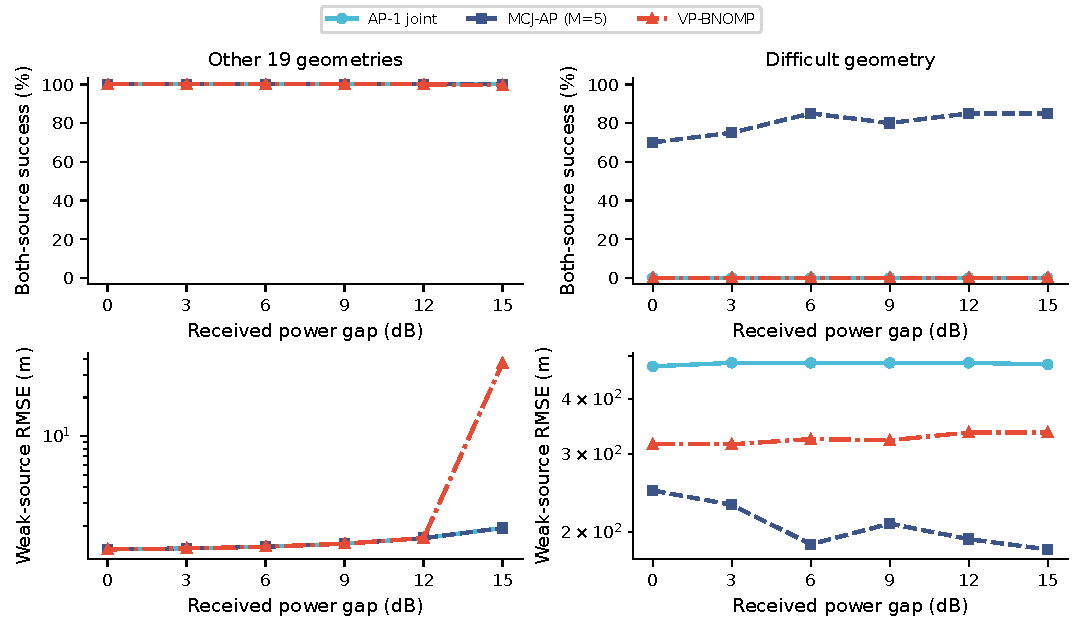
\includegraphics[width=\linewidth]{figures/formal_core.pdf}
\caption{Power-gap results separated into the other 19 configurations (2,280 observations, 380 per gap) and configuration 4 (120 observations, 20 per gap). This post hoc diagnostic grouping retains every observation in the main overall results.}\label{sup:powergroups}
\end{figure}
The other configurations show AP weak-source RMSE increasing from 1.31 to 1.93 m across the power sweep. VP has two 15 dB failures outside configuration 4, so its high-gap RMSE retains a tail. Configuration 4 drives the nonmonotone overall RMSE pattern. Each gap uses the same configurations; the pattern does not arise from changing geometry between power bins.

\begin{figure}[pos=H]\centering
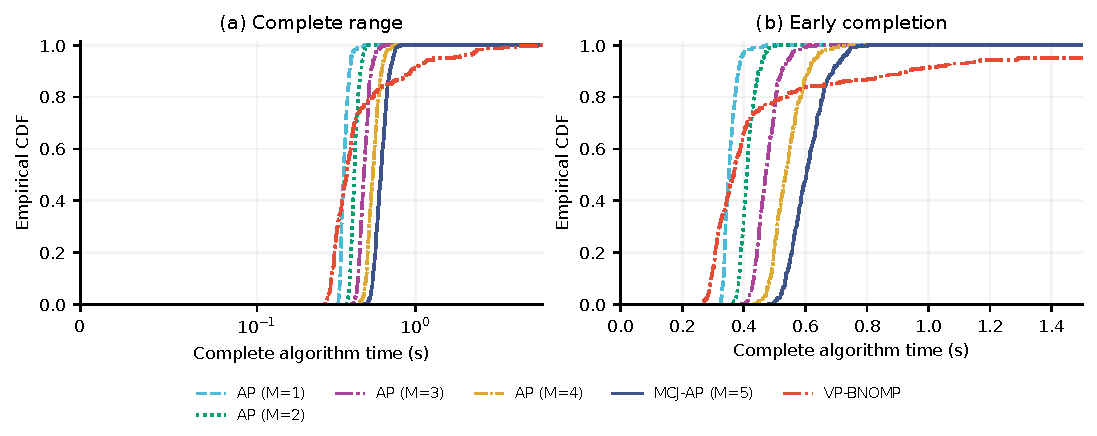
\includegraphics[width=\linewidth]{figures/assignment_cost_20261019/candidate_time_cdf.pdf}
\caption{Complete-runtime CDFs for AP with one to five candidates and VP-BNOMP, 240 observations per method in the same interleaved batch.}\label{sup:candidatetime}
\end{figure}
VP median runtime is 0.3674 s versus 0.3514 s for one-candidate AP. Its P95 is 1.3147 s, exceeding the 0.7201 s of five-candidate AP. Among the 228 observations where both VP and five-candidate AP succeed, VP is faster in 197. Five-candidate AP recovers the other 12 observations. These paired facts describe the observed runtime--recovery trade-off; the single-candidate reference remains part of the comparison.

\begin{figure}[pos=H]\centering
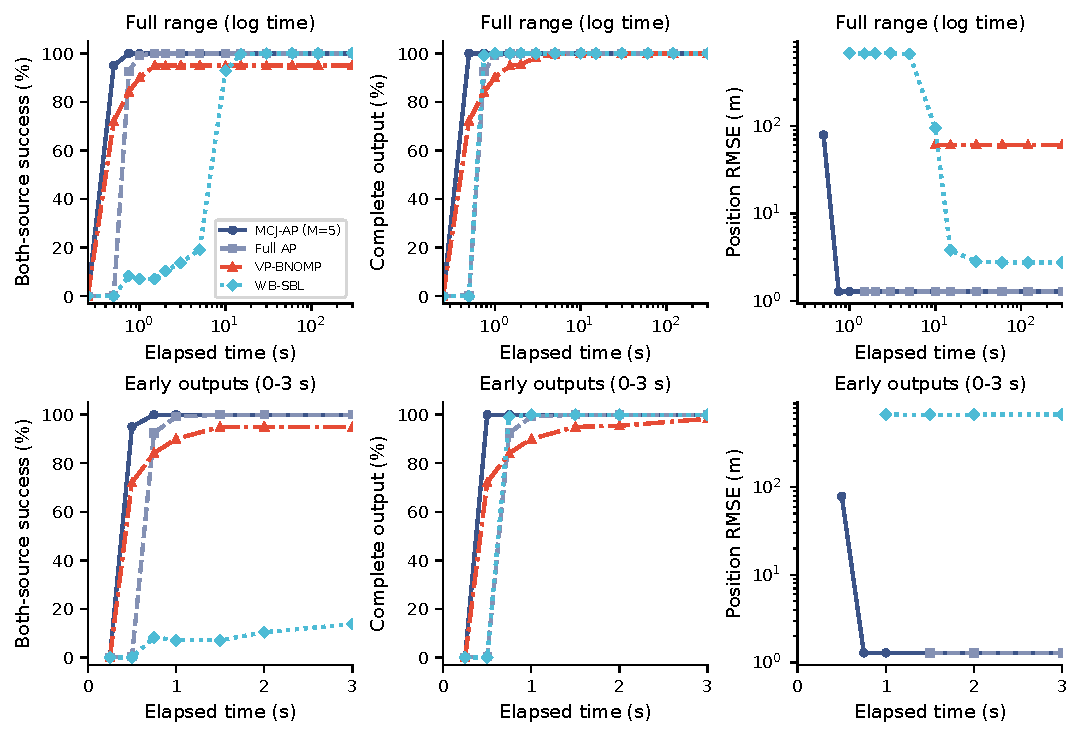
\includegraphics[width=\linewidth]{figures/formal_time.pdf}
\caption{Saved output trajectories on 240 observations. Upper panels span 0.25--300 s logarithmically; lower panels enlarge 0--3 s. Columns show two-source success, complete-output fraction and pooled RMSE. No output counts as unsuccessful; pooled RMSE is shown after every observation has an output.}\label{sup:time}
\end{figure}
Five-candidate AP, full AP and SBL first reach complete success at saved times of 0.75, 1.5 and 30 s, respectively. The connected curves interpolate saved checkpoints and do not define new deployable stopping rules. VP publishes only a final complete output in this recorded batch, so its curve does not represent all internal cycles.

\begin{figure}[pos=H]\centering
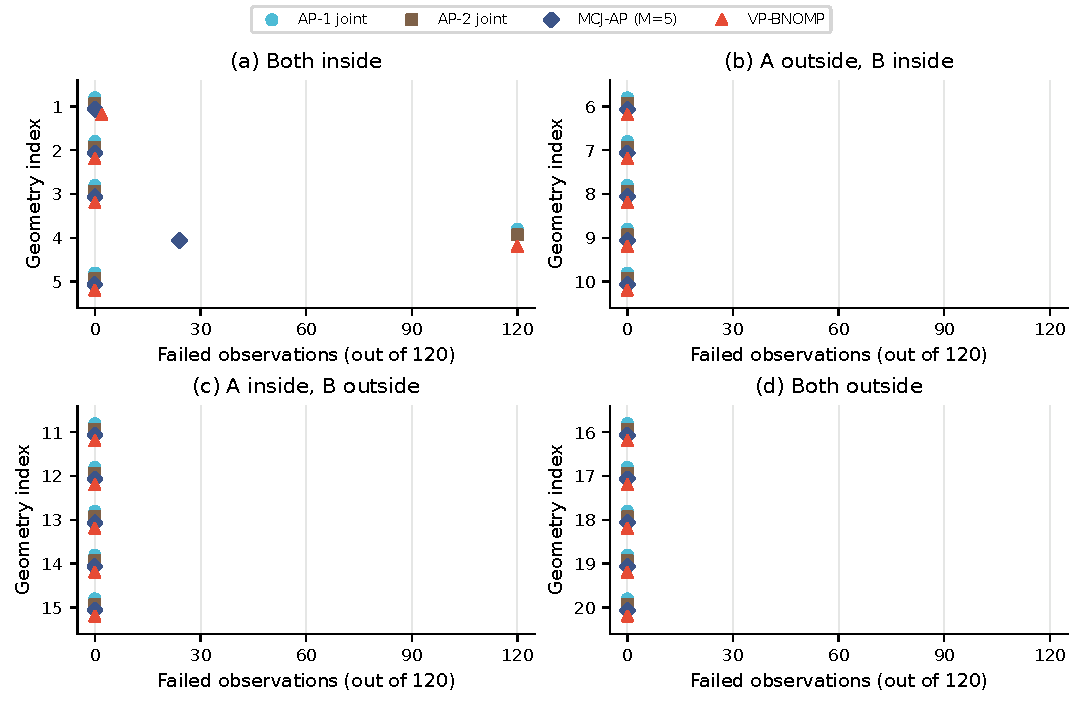
\includegraphics[width=\linewidth]{figures/formal_layouts.pdf}
\caption{Two-source failure counts by original source configuration, 120 observations each. All failures are retained in the main tables and CDFs.}\label{sup:failures}
\end{figure}
All 96 additional five-candidate recoveries occur in configuration 4 across 18 realizations. Its 24 remaining failures involve six realizations, which may overlap the recovered-realization set through different power conditions. Saved branch evaluation finds no successful branch lost by final residual selection. VP reduces configuration-4 weak-source RMSE from the single-candidate AP's 479.66 m to 325.07 m but does not reach the success tolerance there. In the other 19 configurations, its two failures in configuration 1 at 15 dB produce 15.25 m weak-source RMSE, compared with about 1.52 m for AP.

\section{Evidence and timing interpretation}
The formal curvature batch uses the same 240 observations as two historical VP cohorts. Audit comparisons cover 480 old/new pairs: input identities, truths, frozen configurations, positions, native objectives, computation counts, stopping reasons and saved position/objective histories agree within the registered numerical tolerances. Absolute runtimes differ between batches. The available records do not establish which environmental fluctuation caused the difference. Accordingly, each reported speedup uses its own same-batch pair, and absolute times are not combined to form additional speedup claims.

In the curvature pair, mean core times are 5.5483 and 0.8987 s; recording plus final checks average about 0.0254 and 0.0059 s. VP--VP is faster in 170/240 observations. The 83.77\% saving interval resamples realizations within the 20 fixed configurations, keeps six power conditions together and uses 4,000 bootstrap draws with seed 20261020. It describes uncertainty conditional on these configurations and measurements, rather than arbitrary unseen geometries or execution environments.

The 90 VP failures at new positions comprise 30, 25, 30 and five observations in one-based configurations 8, 9, 14 and 15. Every gap has 15 failures; all five realizations are represented. Of these failures, 55 affect only B, 33 both sources and two only A. All fail at the first saved full pair and none has a later saved success. Their final objectives exceed AP's and they stop by energy stability, with mean runtime 1.448 s versus 0.959 s for successful VP observations. These findings exclude a discarded saved successful output or a safety-limit truncation as the explanation in this batch. Since the first full saved state follows one two-source cycle, the records do not isolate the first failed discovery or local update.

\FloatBarrier
\bibliographystyle{\PaperRoot template/cas-model2-names}
\bibliography{\PaperRoot references/references}
\end{document}
